\chapter[Sprint III]{Study and Implementation of Sprint III: Project Management}


\section{Introduction}

Sprint III focuses on implementing comprehensive project management functionality within the UML diagram generation platform. This sprint represents a crucial milestone in the application's development, introducing essential features that enable users to organize, manage, and maintain their UML projects effectively. The project management module serves as the foundation for user workflow organization, providing capabilities for project creation, modification, visualization, and data export. This sprint emphasizes user-centric design principles while ensuring robust backend functionality to support scalable project operations.

\section{Sprint Planning}

The sprint planning phase involved careful analysis of user requirements and technical specifications to deliver a comprehensive project management system. The planning process focused on implementing core CRUD operations while incorporating advanced features such as diagram export and project sharing capabilities.

\subsection{Objectives of Sprint III}

The primary objectives of Sprint III include implementing a complete project management system that allows users to efficiently organize their UML diagram projects. Key goals encompass enabling project creation with customizable parameters, providing intuitive project browsing and viewing capabilities, implementing secure project modification features, ensuring safe project deletion with appropriate confirmations, and developing a robust export system for project diagrams in compressed formats. Additionally, the sprint aims to establish a foundation for future collaboration features through preliminary sharing mechanisms.

\subsection{Backlog of Sprint III}

The Sprint III backlog comprises five essential user stories that form the core of the project management functionality:

\begin{itemize}
\item \textbf{User Story 3.1}: As a user, I want to create new projects to organize my UML diagrams systematically (Priority: Must Have)
\item \textbf{User Story 3.2}: As a user, I want to read and view project details to access my existing work (Priority: Must Have)
\item \textbf{User Story 3.3}: As a user, I want to update project details to maintain current and accurate information (Priority: Must Have)
\item \textbf{User Story 3.4}: As a user, I want to delete projects to manage my workspace efficiently (Priority: Must Have)
\item \textbf{User Story 3.5}: As a user, I want to download project diagrams in appropriate formats compressed in a zip file for offline access and sharing (Priority: Must Have)
\end{itemize}

\section{Analyse}

The analysis phase involved comprehensive examination of user requirements and system specifications to design an optimal project management solution. This phase included detailed use case modeling and requirement specification to ensure all functional aspects are properly addressed.

\subsection{Use case diagram for sprint III}

\begin{figure}[H]
\centering
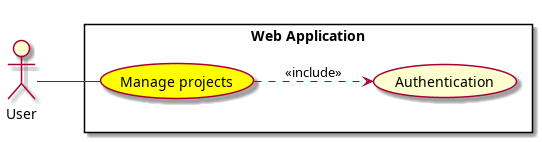
\includegraphics[width=0.8\textwidth]{conception/SprintIII/use_case_diagrams/use_case_diagram_of_SprintIII.png}
\caption{Use case diagram for Sprint III - Project Management}
\label{fig:use_case_sprint3}
\end{figure}

The use case diagram illustrates the complete scope of project management functionality, showing the interactions between users and the system across all implemented features. The diagram demonstrates the comprehensive nature of the project management module and its integration with the overall system architecture.

\subsection{Refined use case "Manage projects"}

\begin{figure}[H]
\centering
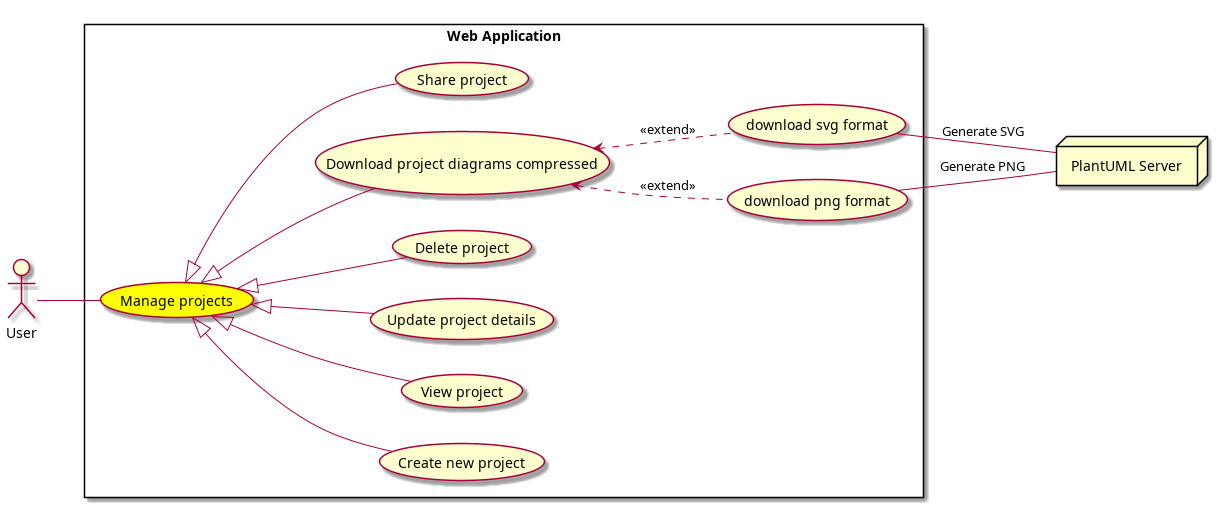
\includegraphics[width=0.9\textwidth]{conception/SprintIII/use_case_diagrams/refined_use_case_feature_project_management.png}
\caption{Refined use case diagram for project management feature}
\label{fig:refined_use_case_project_mgmt}
\end{figure}

\subsubsection{Use case}

The refined use case diagram provides detailed visualization of the project management feature, showing the relationships between different use cases and their extensions. This diagram serves as the foundation for understanding the complete functional scope of the project management system.

\subsubsection{Textual description of use case "Create new project"}

\begin{table}[H]
\centering
\caption{Textual description of "Create new project" use case}
\label{tab:create_project_usecase}
\begin{tabular}{|p{3cm}|p{10cm}|}
\hline
\textbf{Field} & \textbf{Description} \\
\hline
Use Case Name & Create new project \\
\hline
Use Case ID & UC-3.1 \\
\hline
Brief Description & Allows users to create a new project with specified details and initial configuration \\
\hline
Primary Actor & User \\
\hline
Preconditions & User must be authenticated and have access to the project creation interface \\
\hline
Main Flow & 1. User accesses project creation form \newline 2. User enters project name and description \newline 3. User selects project type and initial settings \newline 4. System validates input data \newline 5. System creates new project with unique identifier \newline 6. System displays success confirmation \newline 7. User is redirected to project dashboard \\
\hline
Postconditions & New project is created and available in user's project list \\
\hline
Alternative Flows & A1. Invalid input data: System displays validation errors and prompts for correction \\
\hline
Exception Flows & E1. System error: Display error message and maintain form data \\
\hline
\end{tabular}
\end{table}

\subsubsection{Textual description of use case "View project"}

\begin{table}[H]
\centering
\caption{Textual description of "View project" use case}
\label{tab:view_project_usecase}
\begin{tabular}{|p{3cm}|p{10cm}|}
\hline
\textbf{Field} & \textbf{Description} \\
\hline
Use Case Name & View project \\
\hline
Use Case ID & UC-3.2 \\
\hline
Brief Description & Enables users to view detailed information about existing projects including diagrams and metadata \\
\hline
Primary Actor & User \\
\hline
Preconditions & User must be authenticated and have access to at least one project \\
\hline
Main Flow & 1. User accesses project list interface \newline 2. User selects specific project to view \newline 3. System retrieves project details and associated diagrams \newline 4. System displays project information in organized layout \newline 5. User can navigate through different project sections \newline 6. User can view individual diagrams within the project \\
\hline
Postconditions & User has viewed project details and can proceed with other actions \\
\hline
Alternative Flows & A1. Empty project: System displays message indicating no diagrams are available \\
\hline
Exception Flows & E1. Project not found: Display appropriate error message \newline E2. Access denied: Redirect to authentication or show permission error \\
\hline
\end{tabular}
\end{table}

\subsubsection{Textual description of use case "Update project details"}

\begin{table}[H]
\centering
\caption{Textual description of "Update project details" use case}
\label{tab:update_project_usecase}
\begin{tabular}{|p{3cm}|p{10cm}|}
\hline
\textbf{Field} & \textbf{Description} \\
\hline
Use Case Name & Update project details \\
\hline
Use Case ID & UC-3.3 \\
\hline
Brief Description & Allows users to modify existing project information including name, description, and settings \\
\hline
Primary Actor & User \\
\hline
Preconditions & User must be authenticated and have ownership/edit permissions for the target project \\
\hline
Main Flow & 1. User accesses project edit interface \newline 2. System displays current project information in editable form \newline 3. User modifies desired fields \newline 4. User submits changes \newline 5. System validates updated information \newline 6. System saves changes to database \newline 7. System displays success confirmation \newline 8. Updated information is reflected in project views \\
\hline
Postconditions & Project details are updated and changes are persisted in the system \\
\hline
Alternative Flows & A1. No changes made: System displays message and returns to project view \newline A2. Validation errors: System highlights errors and prompts for correction \\
\hline
Exception Flows & E1. Concurrent modification: Display conflict resolution options \newline E2. Database error: Show error message and maintain user input \\
\hline
\end{tabular}
\end{table}

\subsubsection{Textual description of use case "Delete project"}

\begin{table}[H]
\centering
\caption{Textual description of "Delete project" use case}
\label{tab:delete_project_usecase}
\begin{tabular}{|p{3cm}|p{10cm}|}
\hline
\textbf{Field} & \textbf{Description} \\
\hline
Use Case Name & Delete project \\
\hline
Use Case ID & UC-3.4 \\
\hline
Brief Description & Enables users to permanently remove projects from their workspace with appropriate safety measures \\
\hline
Primary Actor & User \\
\hline
Preconditions & User must be authenticated and have ownership/delete permissions for the target project \\
\hline
Main Flow & 1. User selects project for deletion \newline 2. System displays confirmation dialog with project details \newline 3. User confirms deletion intent \newline 4. System performs additional confirmation for critical projects \newline 5. System removes project and associated data from database \newline 6. System cleans up related files and resources \newline 7. System displays deletion confirmation \newline 8. User is redirected to updated project list \\
\hline
Postconditions & Project and all associated data are permanently removed from the system \\
\hline
Alternative Flows & A1. User cancels deletion: Return to project view without changes \newline A2. Shared project: Display warning about impact on other users \\
\hline
Exception Flows & E1. System error during deletion: Display error message and maintain project data \newline E2. Referenced project: Show dependencies and require resolution \\
\hline
\end{tabular}
\end{table}

\subsubsection{Textual description of use case "Download project diagrams compressed"}

\begin{table}[H]
\centering
\caption{Textual description of "Download project diagrams compressed" use case}
\label{tab:download_project_usecase}
\begin{tabular}{|p{3cm}|p{10cm}|}
\hline
\textbf{Field} & \textbf{Description} \\
\hline
Use Case Name & Download project diagrams compressed \\
\hline
Use Case ID & UC-3.5 \\
\hline
Brief Description & Allows users to export all project diagrams in various formats packaged in a compressed zip file \\
\hline
Primary Actor & User \\
\hline
Preconditions & User must be authenticated, have access to the project, and project must contain at least one diagram \\
\hline
Main Flow & 1. User accesses project export interface \newline 2. User selects desired export formats (PNG, SVG, PDF) \newline 3. User initiates download process \newline 4. System generates diagrams in selected formats \newline 5. System creates compressed zip file containing all diagrams \newline 6. System initiates file download to user's device \newline 7. User receives compressed file with organized diagram collection \\
\hline
Postconditions & User has downloaded a compressed file containing all project diagrams in selected formats \\
\hline
Alternative Flows & A1. Large project: System displays progress indicator during generation \newline A2. Selective export: User can choose specific diagrams to include \\
\hline
Exception Flows & E1. Generation error: Display error message and suggest alternative formats \newline E2. File size limit: Warn user and offer options to reduce file size \\
\hline
\end{tabular}
\end{table}

\section{Conception}

The conception phase involved detailed design of system interactions and workflow processes for each project management feature. Sequence diagrams were developed to illustrate the communication patterns between system components and ensure proper implementation of business logic.

\subsection{Sequence diagram of use case}

The following sequence diagrams illustrate the detailed interactions between system components for each implemented use case:

\begin{figure}[H]
\centering
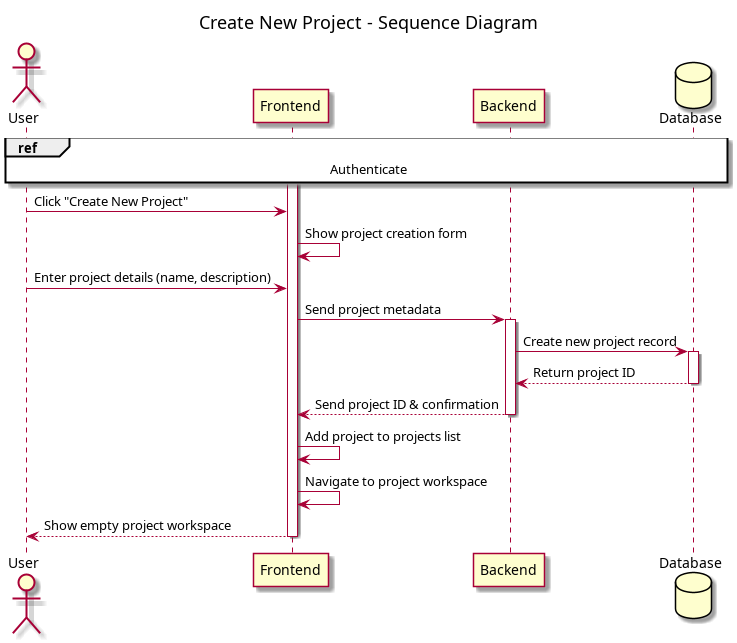
\includegraphics[width=\textwidth]{conception/SprintIII/sequence_diagrams/sequence_projectManagement_3_1_CreateNewProject.png}
\caption{Sequence diagram for Create New Project use case}
\label{fig:seq_create_project}
\end{figure}

\begin{figure}[H]
\centering
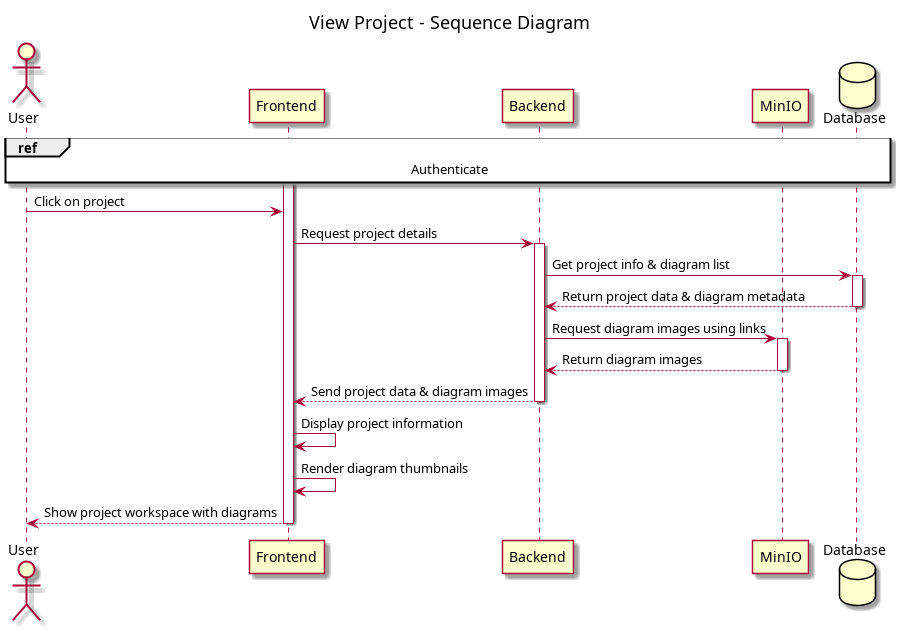
\includegraphics[width=\textwidth]{conception/SprintIII/sequence_diagrams/sequence_projectManagement_3_2_ViewProjectDetails.png}
\caption{Sequence diagram for View Project Details use case}
\label{fig:seq_view_project}
\end{figure}

\begin{figure}[H]
\centering
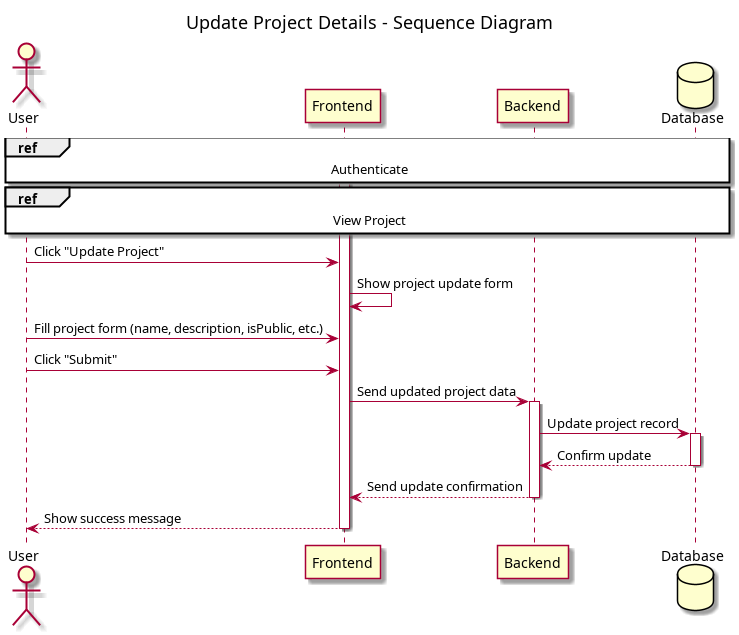
\includegraphics[width=\textwidth]{conception/SprintIII/sequence_diagrams/sequence_projectManagement_3_3_UpdateProjectDetails.png}
\caption{Sequence diagram for Update Project Details use case}
\label{fig:seq_update_project}
\end{figure}

\begin{figure}[H]
\centering
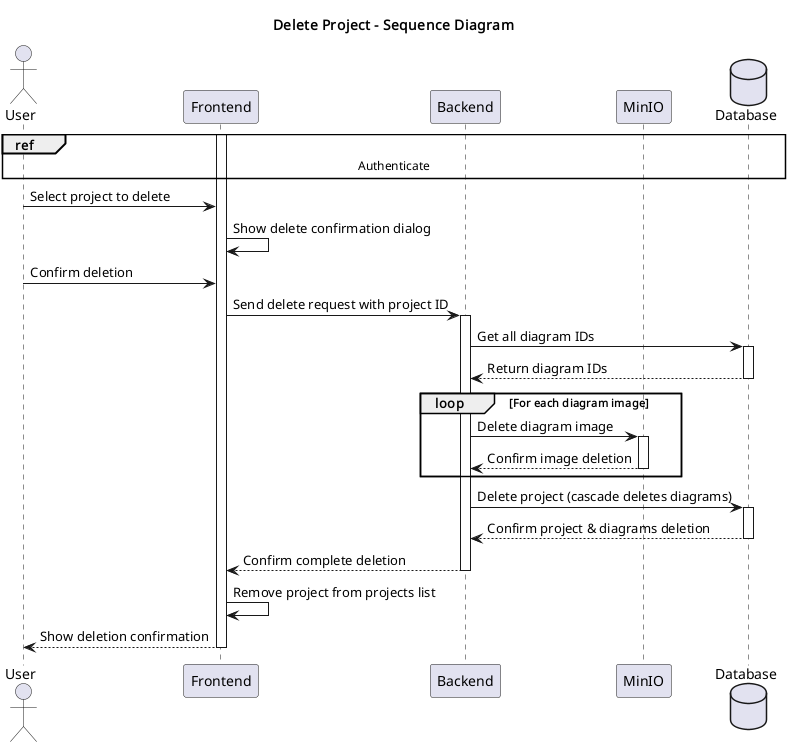
\includegraphics[width=\textwidth]{conception/SprintIII/sequence_diagrams/sequence_projectManagement_3_4_DeleteProject.png}
\caption{Sequence diagram for Delete Project use case}
\label{fig:seq_delete_project}
\end{figure}

\begin{figure}[H]
\centering
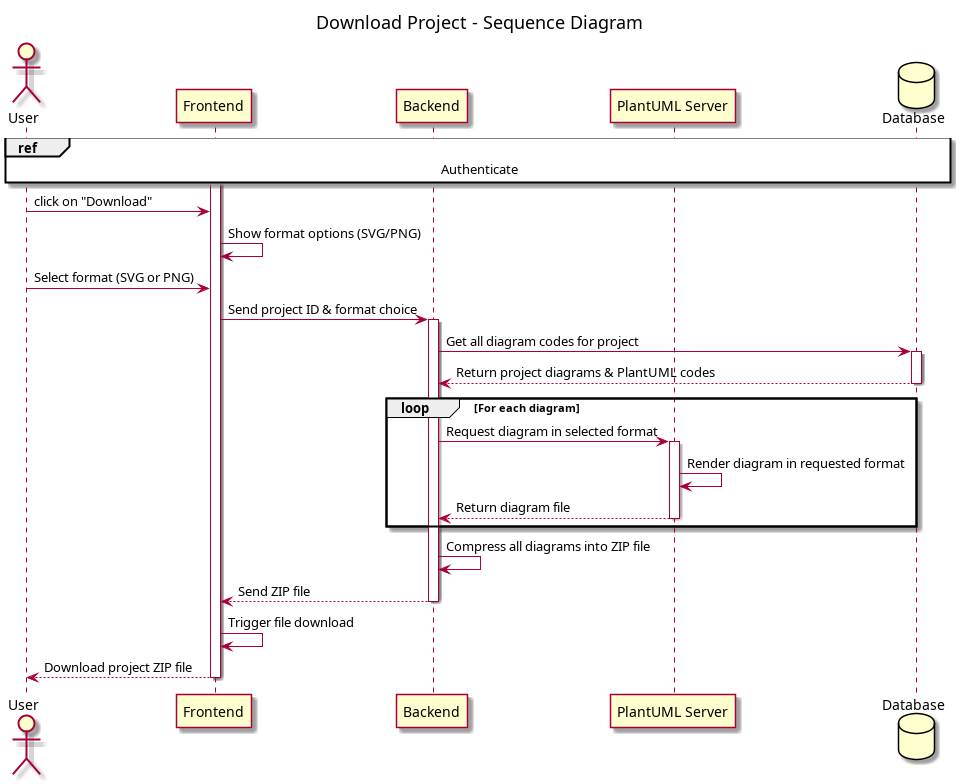
\includegraphics[width=\textwidth]{conception/SprintIII/sequence_diagrams/sequence_projectManagement_3_5_DownloadProjectDiagramsAsZip.png}
\caption{Sequence diagram for Download Project Diagrams as Zip use case}
\label{fig:seq_download_project}
\end{figure}

\begin{figure}[H]
\centering
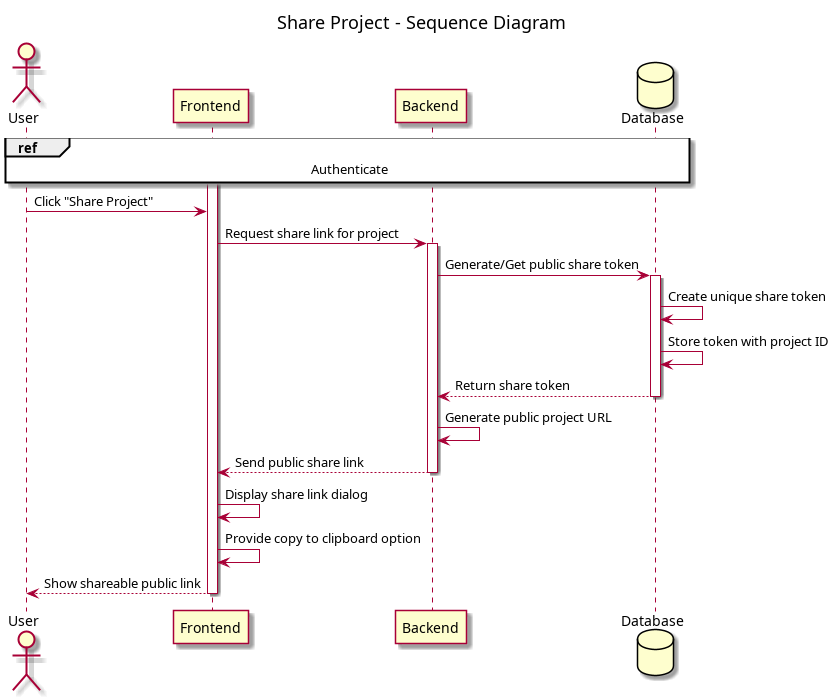
\includegraphics[width=\textwidth]{conception/SprintIII/sequence_diagrams/sequence_projectManagement_3_6_ShareProject.png}
\caption{Sequence diagram for Share Project use case}
\label{fig:seq_share_project}
\end{figure}

\section{Deliverables of Sprint III}

Sprint III successfully delivered a comprehensive project management system with intuitive user interfaces and robust functionality. The implementation includes all planned features with additional enhancements for improved user experience.

\begin{figure}[H]
\centering
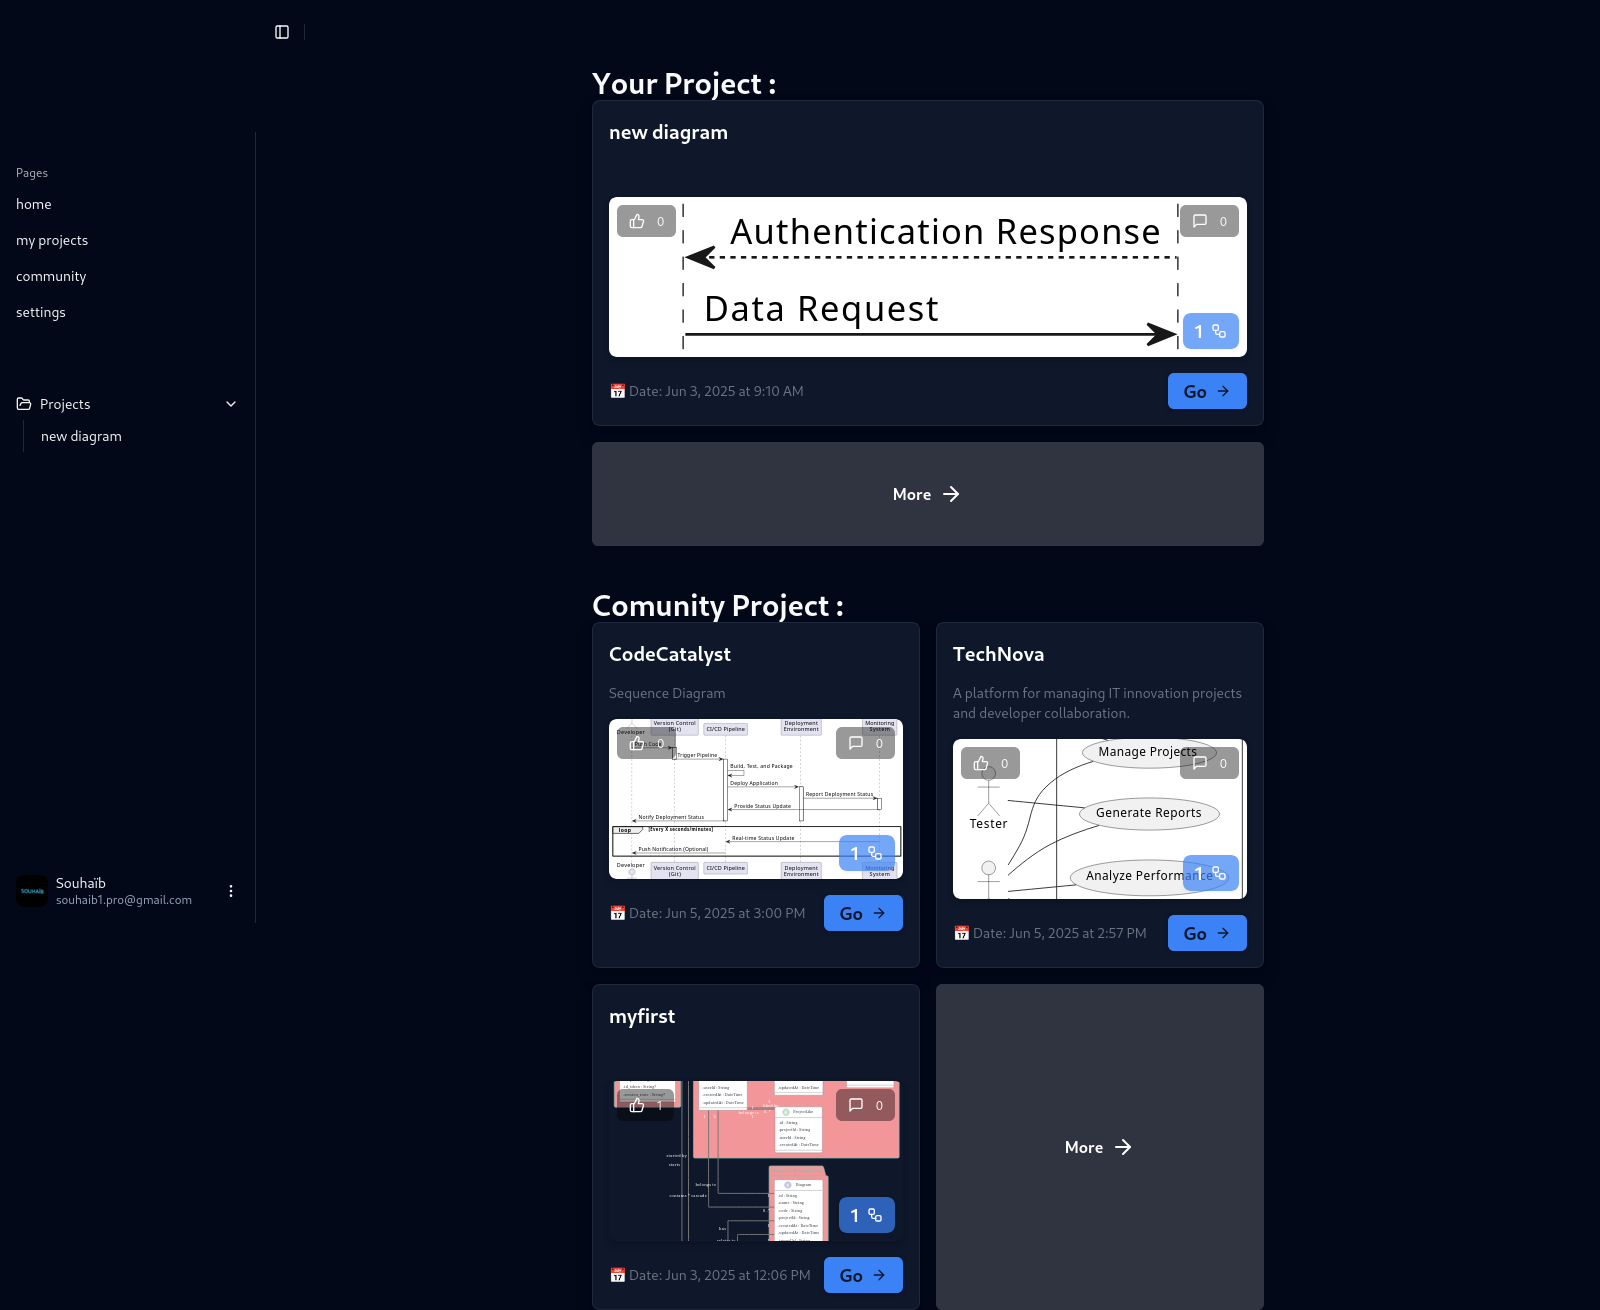
\includegraphics[width=0.8\textwidth]{screenshots/home.png}
\caption{Home page showing project overview and navigation}
\label{fig:home_page}
\end{figure}

\begin{figure}[H]
\centering
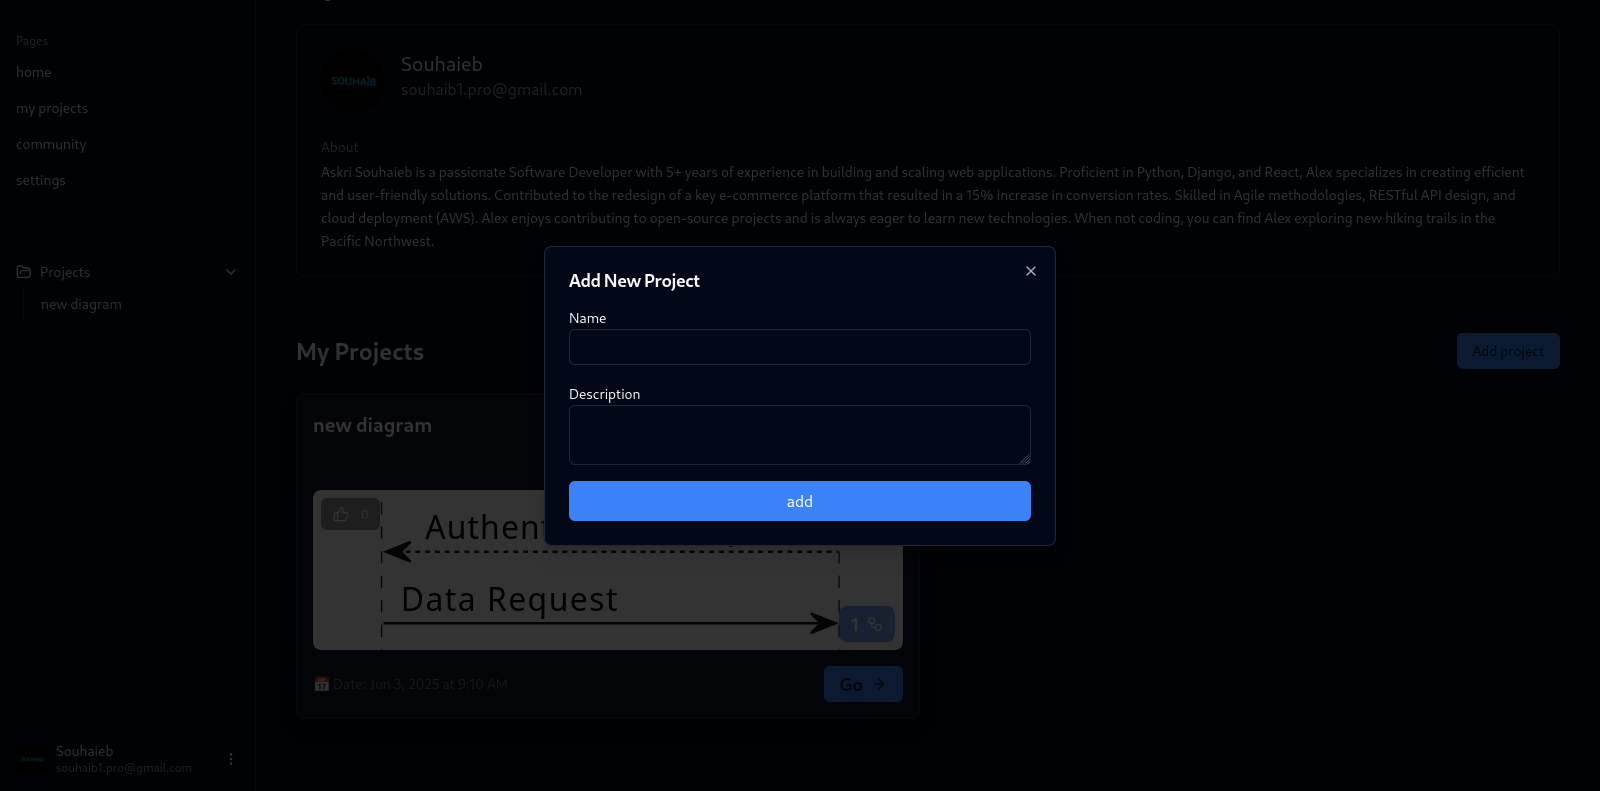
\includegraphics[width=0.8\textwidth]{screenshots/add-project.png}
\caption{Add project interface with form validation and user guidance}
\label{fig:add_project}
\end{figure}

\begin{figure}[H]
\centering
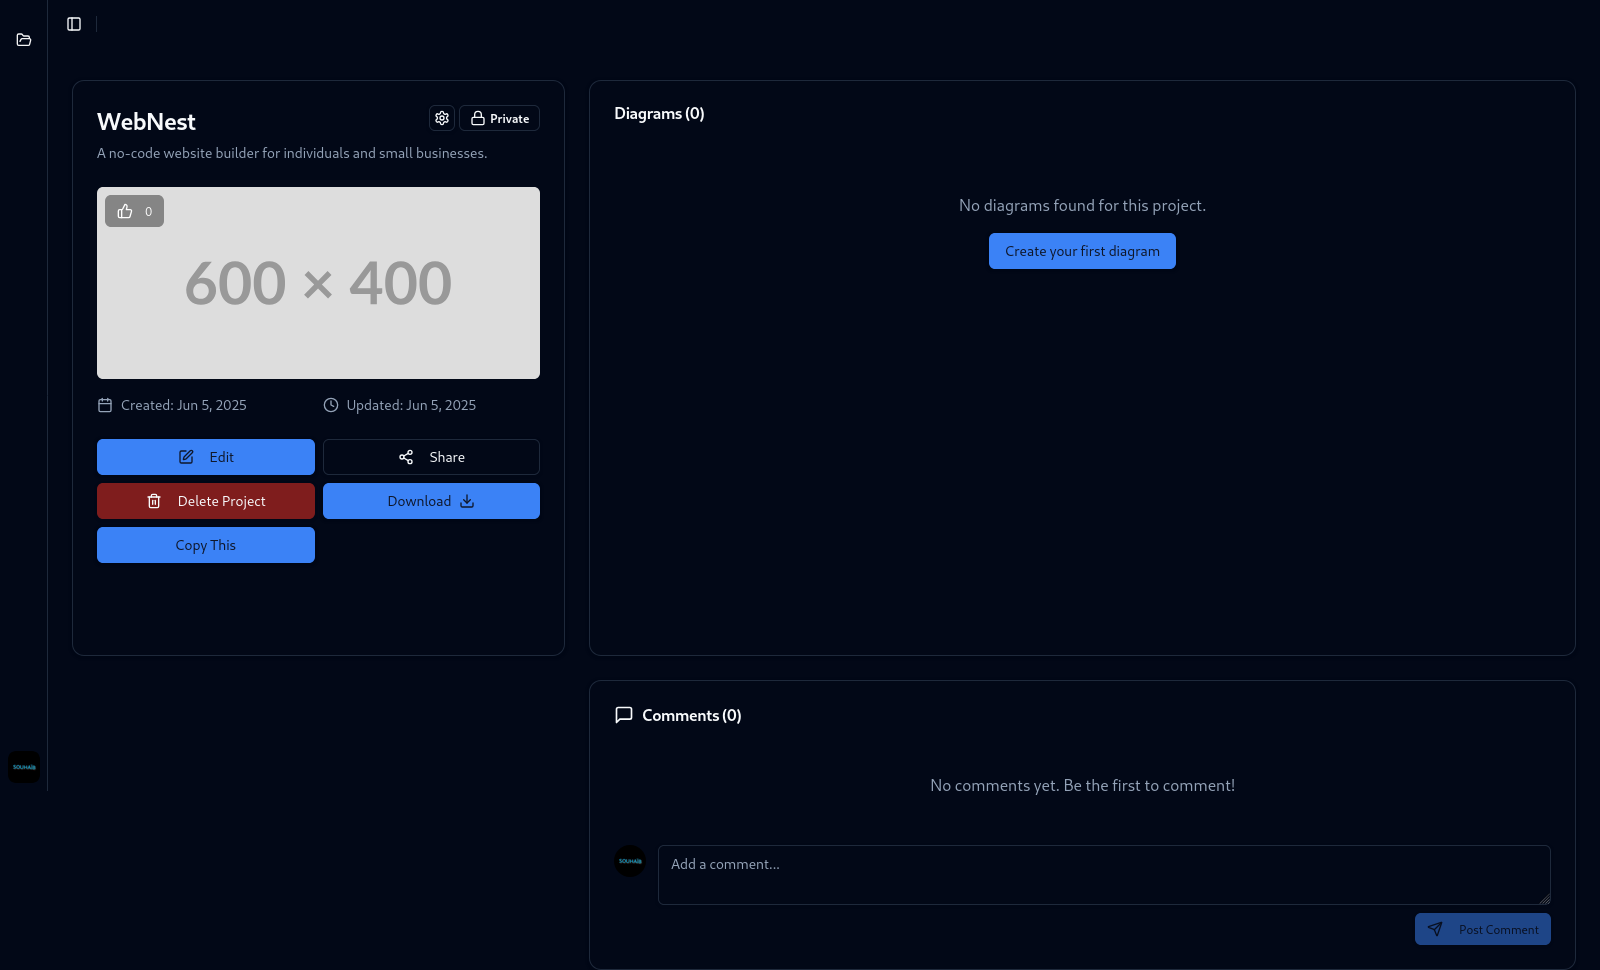
\includegraphics[width=0.8\textwidth]{screenshots/project-page.png}
\caption{Project details page displaying comprehensive project information}
\label{fig:project_page}
\end{figure}

\begin{figure}[H]
\centering
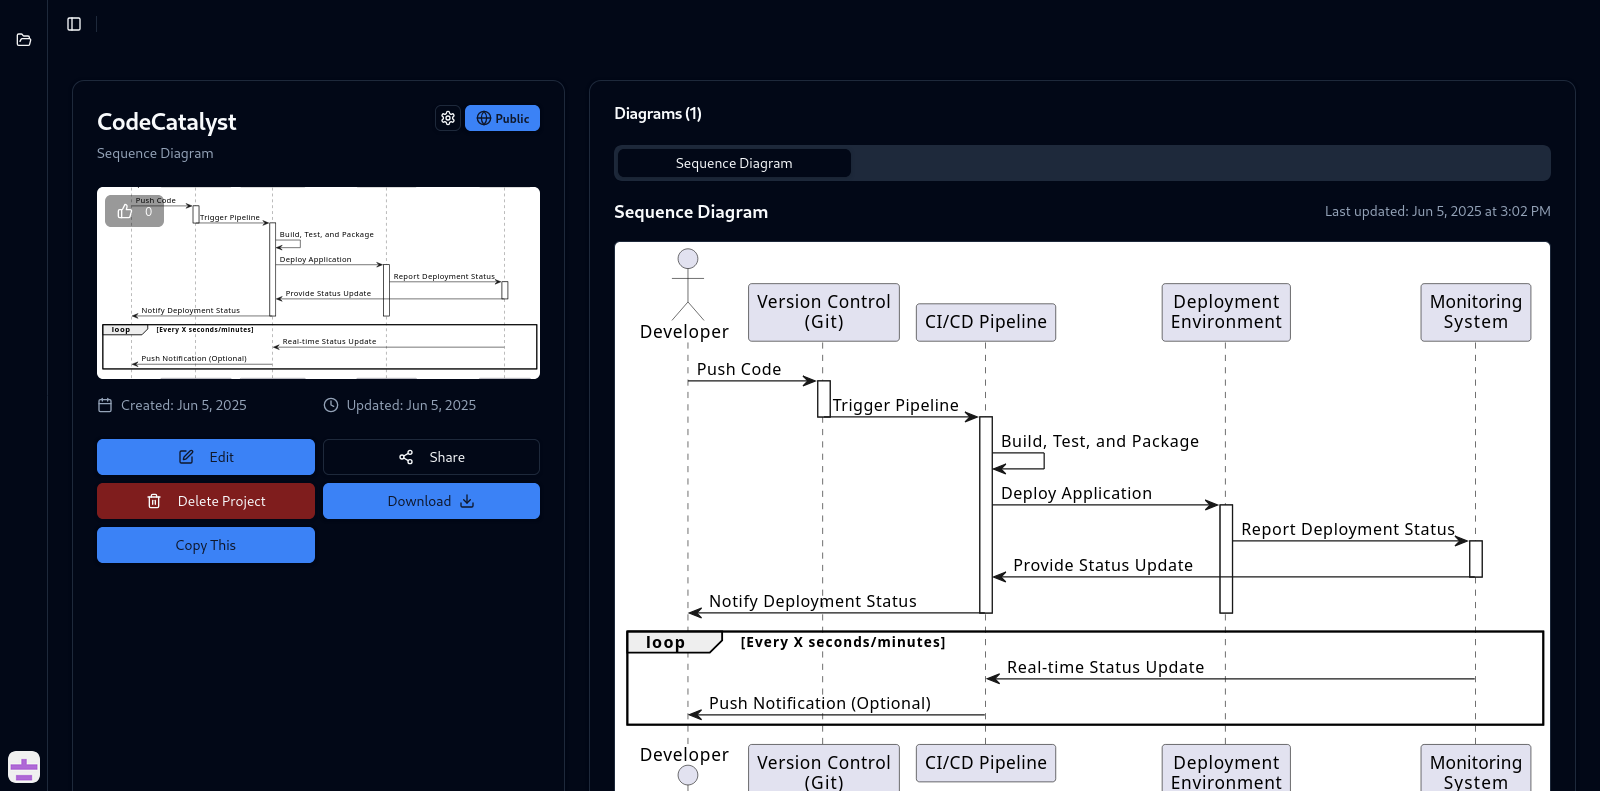
\includegraphics[width=0.8\textwidth]{screenshots/project-page2.png}
\caption{Extended project view with diagram management capabilities}
\label{fig:project_page2}
\end{figure}

\begin{figure}[H]
\centering
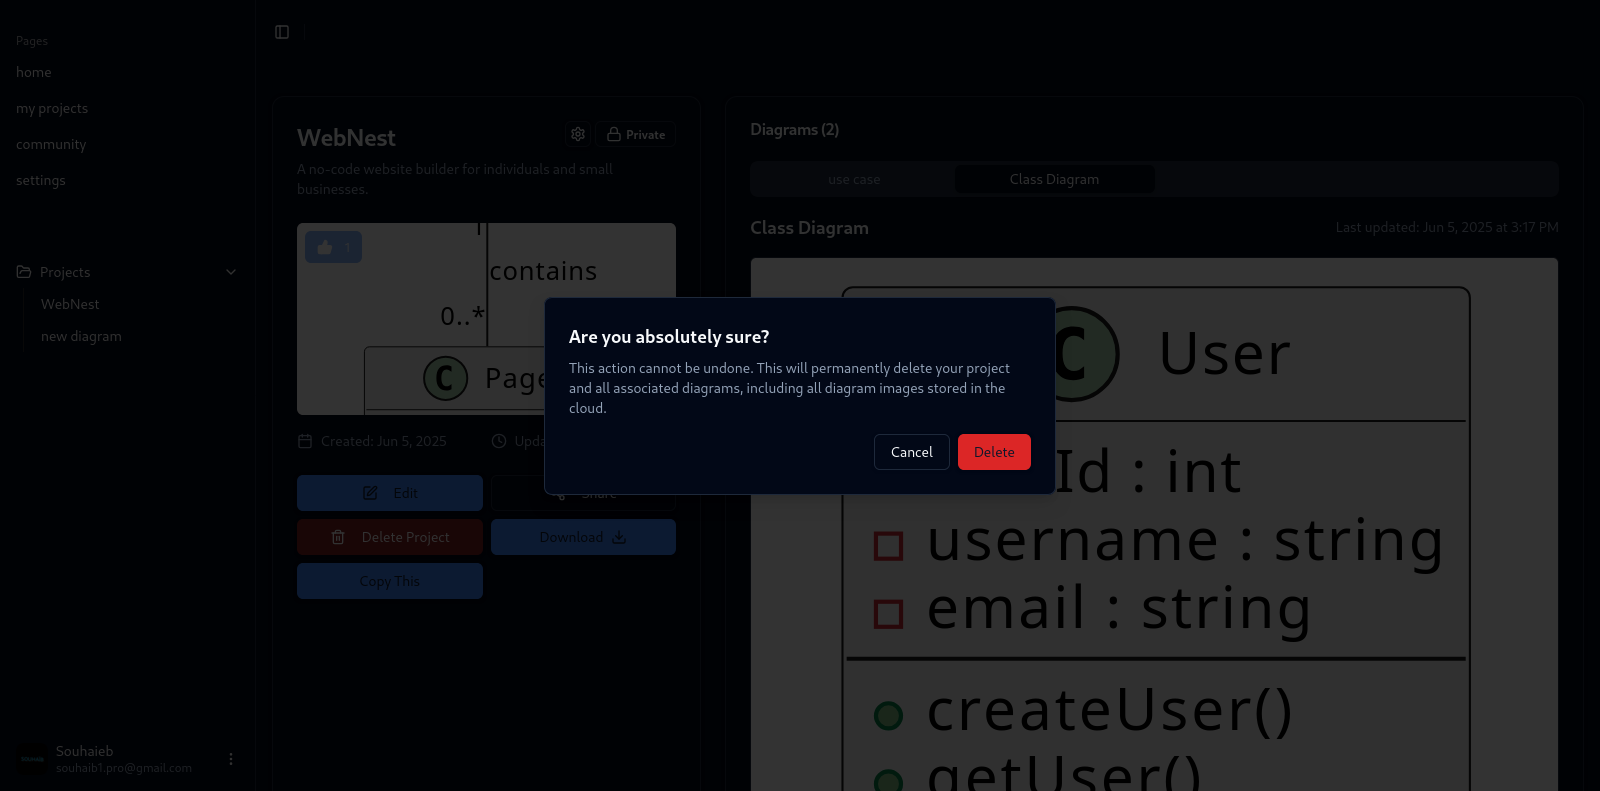
\includegraphics[width=0.8\textwidth]{screenshots/delate.png}
\caption{Project deletion confirmation dialog with safety measures}
\label{fig:delete_confirmation}
\end{figure}

\begin{figure}[H]
\centering
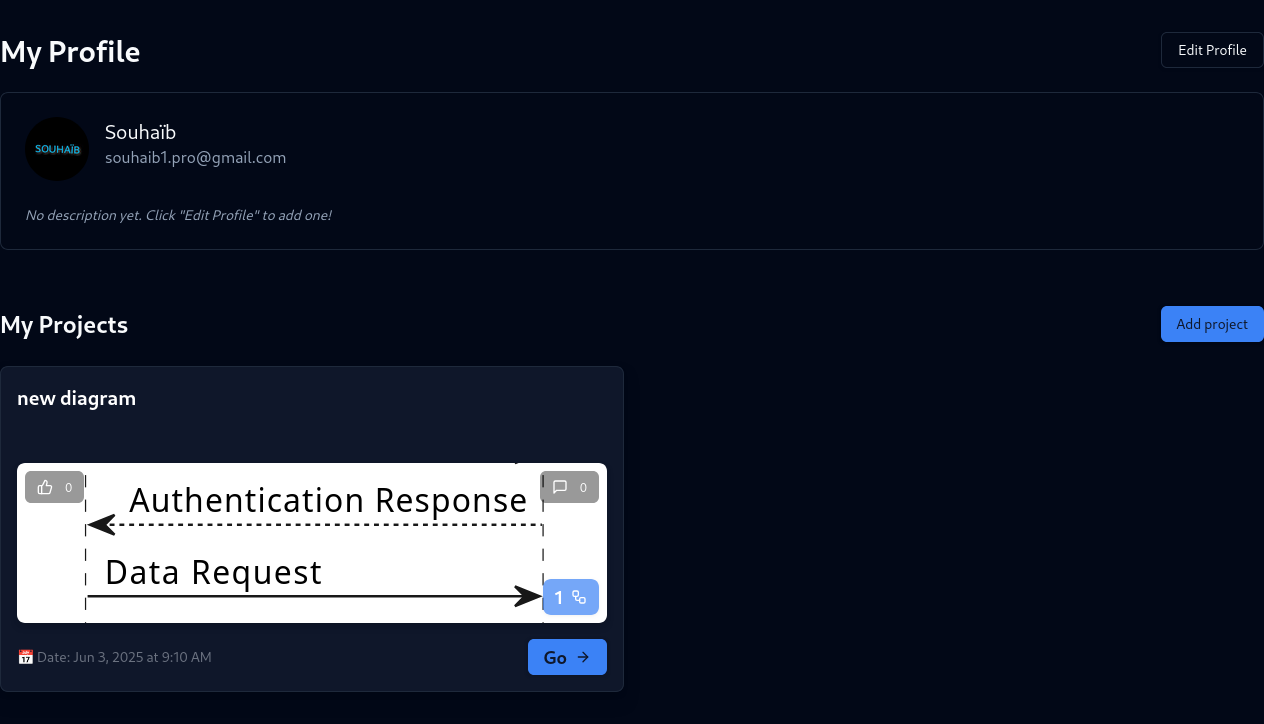
\includegraphics[width=0.8\textwidth]{screenshots/me.png}
\caption{User profile and project management dashboard}
\label{fig:user_profile}
\end{figure}

\section{Retrospective of Sprint III}

Sprint III achieved significant success in implementing a comprehensive project management system that exceeded initial expectations. The team effectively collaborated to deliver all planned features while maintaining high code quality and user experience standards. Key achievements include successful implementation of all CRUD operations, robust export functionality, and intuitive user interfaces. The sprint demonstrated strong technical execution and effective requirement analysis. Areas for improvement include enhanced error handling mechanisms and performance optimization for large projects. The foundation established in this sprint provides excellent groundwork for future enhancements and collaboration features.

\section{Conclusion}

Sprint III successfully established a robust project management foundation for the UML diagram generation platform. The implemented features provide users with comprehensive tools for organizing, managing, and sharing their UML projects effectively. The sprint delivered significant value through intuitive interfaces, reliable functionality, and scalable architecture. The project management module now serves as a central hub for user workflow organization, enabling efficient project lifecycle management. This sprint's achievements position the platform for continued growth and enhanced collaboration capabilities in future development cycles. The successful completion of Sprint III demonstrates the team's ability to deliver complex functionality while maintaining high standards of quality and user experience.